\subsection{Neural Network Model}
%Neural network is a kind of computational model widely used in 
%machine learning, computer science and other research disciplines. 
%Recent research indicates that traditional machine learning methods are not sufficiently capable of extracting suitable features and capturing the non-linear nature of complex tasks. 
%Neural network models are presented as a remedy. 
%Fig. \ref{fig:nn} shows the structure of a typical three-layer neural network. 
%Each connection between (two) neurons can transmit an unidirectional signal with an activating strength that varies with the strength of the connection. 
%As a result, a typical four-layer neural network model can approximate most non-linear functions.
%
We adopt a four-layer neural network model (MLP) with following structure: 
the size of input layer is equal to the dimensionality of $\mathbf{x}$; 
the second layer contains half of it; 
the third is half of the second layer; 
the final output layer contains only one neuron.
The model (NN) takes the same input as before and output a continuous value by the last output layer which is the predicted speed.
%If the combined incoming signals (from potentially many transmitting neurons) are strong enough, the receiving neuron activates and propagates a signal to downstream neurons connected to it.

%\begin{figure}[th!]
%	\centering
%	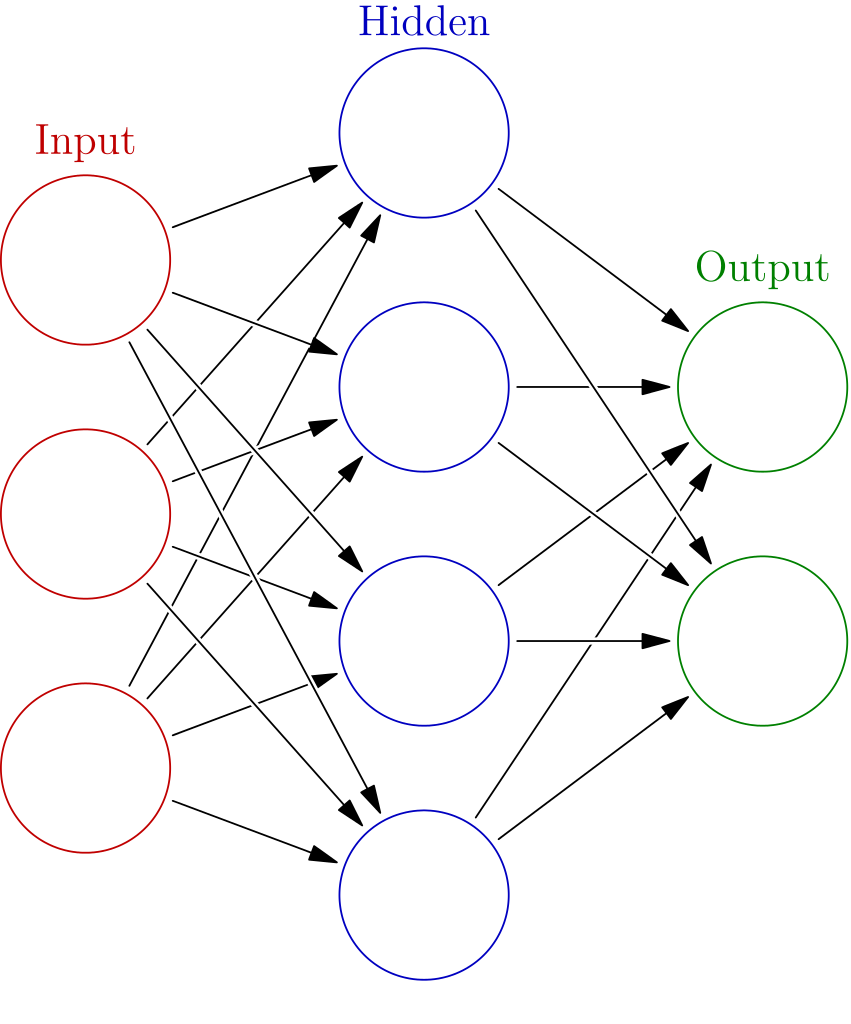
\includegraphics[width=0.3\textwidth]{figures/Colored_neural_network.png}
%	\caption{Structure of a typical neural network}
%	\label{fig:nn}
%\end{figure}

%Moreover, a threshold may govern each connection and neuron, such that the signal must exceed the limit before propagating. 
%Back propagation is the use of forward stimulation to modify connection weights. 
%Training typically requires several thousand cycles of interaction.
%
%In our work, we ...